\documentclass[aspectratio=1610]{beamer}

\usetheme{KTH}
\usepackage{preamble}

% ====>>>>> general

%% The slides should be for the audience, to give them a visual experience.
%% Transitions; one style for the slides and one style for the transitions between topics. e.g. light background, dark text vs. dark background, light text.
%% Don't write too much on the slides.
%% Skip effects.
%% Masking images to direct attention.
%% Simple charts and graphs. If possible, in the same style as the presentation (e.g. fonts, colors).

\begin{document}

% === [ Start page ] ===========================================================

\startpage

\begin{frame}

	\vspace{0.02\textheight}

	\begin{Large}
		Evaluation of Methods for Effective Control Flow Recovery
	\end{Large}

	\vspace{0.1\textheight}

	\begin{small}
		\textit{Robin Eklind}
	\end{small}
\end{frame}

% === [ Introduction ] =========================================================

% ====>>>>> What?

% What?

% Frame problem at a high level.
% 1-3 minutes.

% Key message you wish to communicate. From the perspective of the audience, what will they gain? What can they do with the information?

\normalpage

\begin{frame}
	\frametitle{What?}

	\begin{block}{Control Flow Recovery}
		Analysis of control flow graphs (CFGs) to recover high-level control flow primitives (e.g. \texttt{if}-statement and \texttt{for}-loops) from assembly language or low-level intermediate representations.
	\end{block}
\end{frame}

\begin{frame}
	\frametitle{Control Flow Recovery}

	\begin{figure}[htbp]
		\centering
		\begin{subfigure}[t]{0.27\textwidth}
			\centering
			\lstinputlisting[caption={C source file.}, language=C, style=c, basicstyle=\tiny\ttfamily, breaklines=false, numbers=none]{inc/overview/overview.c}
			\vfill
		\end{subfigure}
		\quad
		\begin{subfigure}[t]{0.52\textwidth}
			\centering
			\lstinputlisting[caption={LLVM IR assembly.}, language=llvm, style=nasm, basicstyle=\tiny\ttfamily, breaklines=false, numbers=none]{inc/overview/overview_mini.ll}
		\end{subfigure}
		\caption{\textit{Reverse compilation}, going from low-level (right) to high-level (left).}
	\end{figure}

\end{frame}

% ====>>>>> Why?

% Why?

% Then go into depth; both intellectual and emotional arguments for the severity of the problem.
% 15-20 minutes if presenting for 1 hour.

\begin{frame}
	\frametitle{Why?}

	\begin{block}{Applications of Control Flow Recovery}
		\begin{itemize}
			\item Malware analysis
			\item Security assessments
			\begin{itemize}
				\item Automated vulnerability scanners
			\end{itemize}
			\item Control-flow aware compiler passes
		\end{itemize}
	\end{block}
\end{frame}

\begin{frame}
	\frametitle{Control-flow Aware Compiler Passes}

	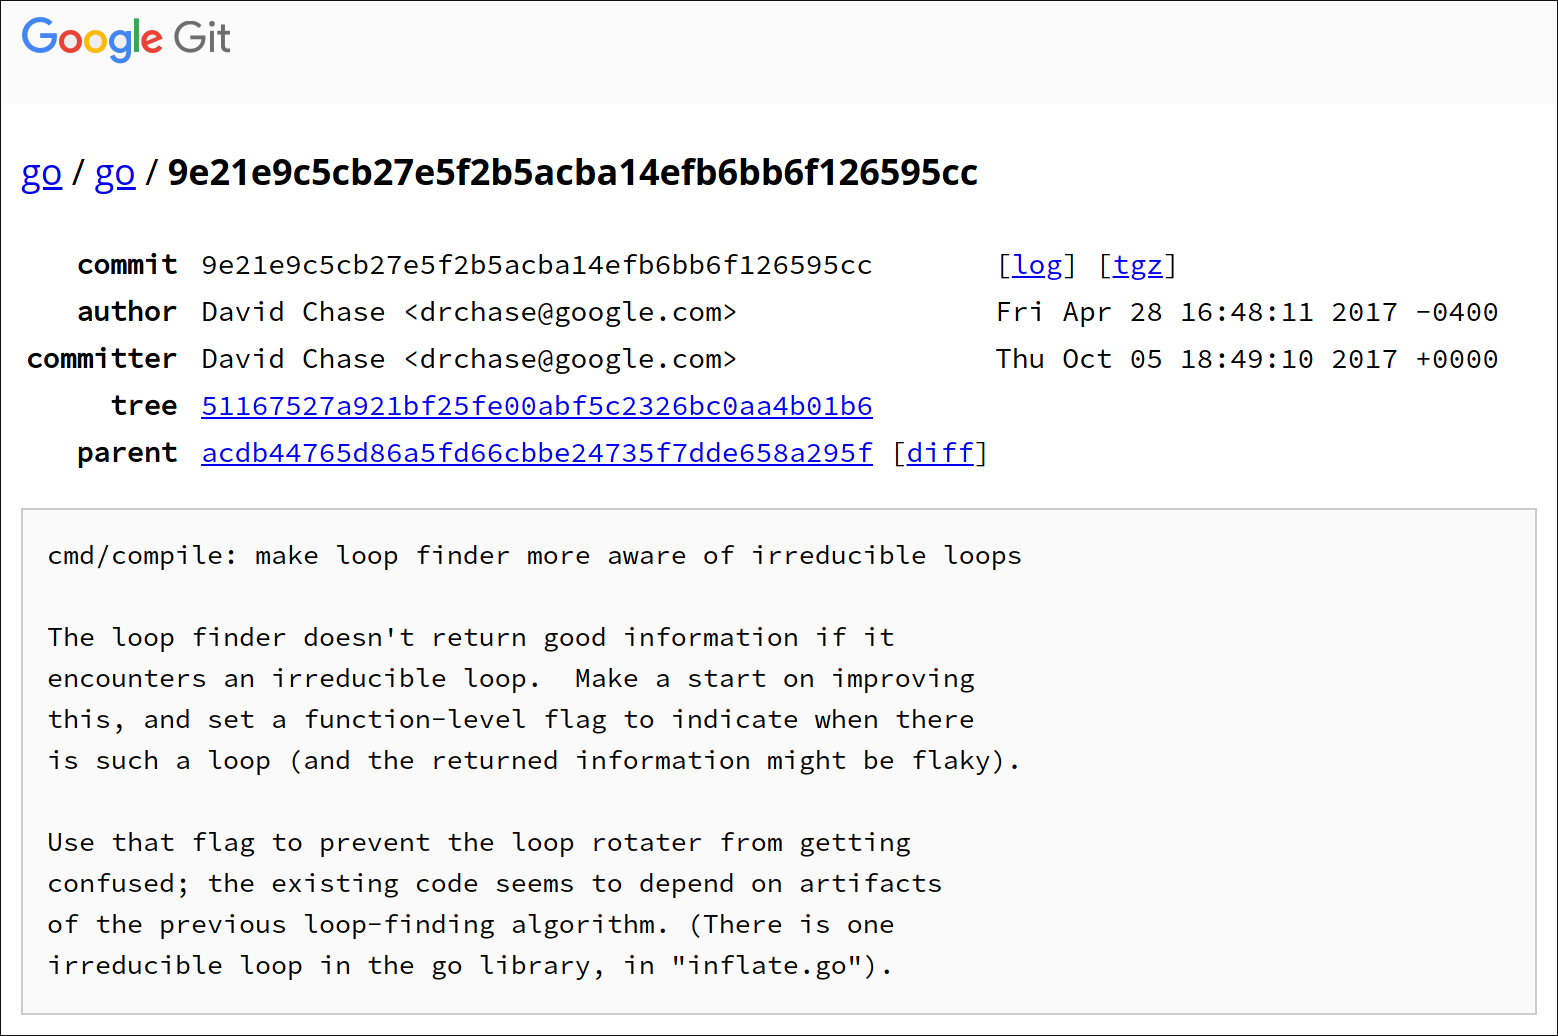
\includegraphics[width=0.8\textwidth]{inc/applications/loop_finder.png}
\end{frame}

% ====>>>>> How?

% How?

% Give solution, including benefits and drawbacks.

\begin{frame}
	\frametitle{How?}

	\begin{block}{Control Flow Recovery Methods}
		\begin{itemize}
			\item baz
			\begin{itemize}
				\item qux
				\item fob
			\end{itemize}
		\end{itemize}
	\end{block}
\end{frame}

\end{document}
